\section{Experiment 1}
In this experiment the aim is to investigate the effect of the training sample size on the performance of the classifier. For this reason the test dataset will be first generated and will not be changed throughout this experiment. The training set, however, will be regenerated on every iteration of the experiment at a range of sizes. As opposed to re-sampling a static training dataset, this regenerated option was used as it would introduce an additional amount of unpredictability to the system. What this means is that as the training set size increases the test error will generally tend to reduce, but the training error  may increase due to this randomness. However in general the mean test and training errors should be seen to converge. In order to account for individual bias in any one training set this experiment was conducted 10 times on each independent training dataset in all sizes $Nd = = [3,5,10,50,100]$ in order to get an average case behaviour of the system with respect to changing training data. In this case the class parameters were used  as instructed resulting in a mean of class 1 as $\mu_{1}$, and the mean of class 2 as $\mu_{1}$, and both classes sharing identical covariance matrices of $\Sigma_{1} = \Sigma_{2}$:

\begin{equation*}
	\mu_{1} =  
	\begin{bmatrix} 
   		1 \\
  		3 \\
	\end{bmatrix}
\end{equation*}

\begin{equation*} 
	\mu_{2} =  
	\begin{bmatrix} 
   		4 \\
  		6 \\
	\end{bmatrix}
\end{equation*}

\begin{equation*}
	\Sigma_{1} = \Sigma_{2} = 
	\begin{bmatrix} 
   		3 & 1  \\
  		1 & 3 \\
	\end{bmatrix}
\end{equation*}

As seen in Figure \ref{fig:SampleDatasets}, some of the datasets generated in this experiment at various sizes of $N_{D}$ which allows us to visualize the overlap between the classes, and how different instances can pose different difficulties in the separability of the data-points in each class from the other.

\begin{figure}[H]
        \centering
        \begin{subfigure}[b]{0.475\textwidth}
            \centering
            \includegraphics[width=\textwidth]{./code/Exp1-results/10iters/Train10.png}
            \caption[]%
            {{\small 10 sample training set}}    
            \label{fig:train10}
        \end{subfigure}
        \hfill
        \begin{subfigure}[b]{0.475\textwidth}  
            \centering 
            \includegraphics[width=\textwidth]{./code/Exp1-results/10iters/Train50.png}
            \caption[]%
            {{\small 50 sample training set}}    
            \label{fig:train50}
        \end{subfigure}
        \vskip\baselineskip
        \begin{subfigure}[b]{0.475\textwidth}   
            \centering 
            \includegraphics[width=\textwidth]{./code/Exp1-results/10iters/Train100.png}
            \caption[]%
            {{\small 100 sample training set}}    
            \label{fig:train100}
        \end{subfigure}
        \quad
        \begin{subfigure}[b]{0.475\textwidth}   
            \centering 
            \includegraphics[width=\textwidth]{./code/Exp1-results/10iters/Test100.png}
            \caption[]%
            {{\small 100 sample test set}}    
            \label{fig:test100}
        \end{subfigure}
        \caption[ ]
        {\small Visualisation of examples of test and training data generated for Experiment 1.} 
        \label{fig:SampleDatasets}
    \end{figure}

On each iteration the training data sets are regenerated, labels are configured appropriately, the model is created using \code{fitcnb()} and a prediction is made with the \code{predict()} function. These are then compared to the ground truth labelled data and an error calculated.

\pagebreak
\subsection{Results \& Discussion}
Seen below, in Figure \ref{fig:exp1} the gradual convergence of the test and training near error percentages. It is important to notice that naturally the test error remains higher to begin with in most cases as the model is more closely fit to the training data when $N_{D}$ is small. As this value grows the errors converge as predicted.

\begin{figure}[H]
	\centering
	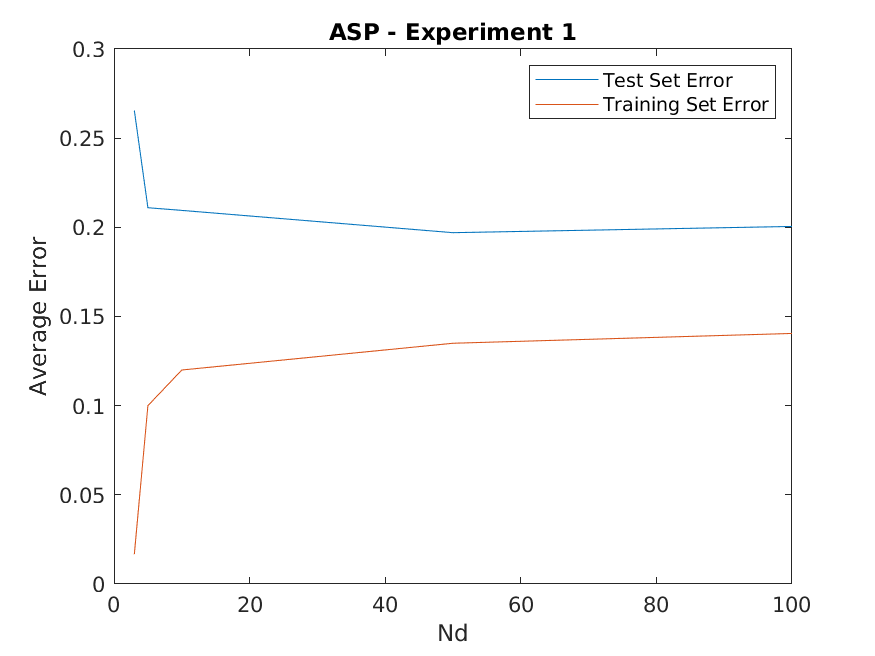
\includegraphics[width=.6\linewidth]{./code/Exp1-results/10iters/ErrorComparison.png}
	\caption{Experiment 1 Results}
	\label{fig:exp1}
\end{figure}

